%
% CryptoWars (TM)
%

\section{CryptoWars\texttrademark -- Quantum cryptography}\index{Quantum key distribution}\index{Quantum cryptography}\index{CryptoWars}\label{sec:cryptowars}

Undoubtedly, quantum technologies will be most impactful (and disruptive!) in the area of information security, something of fundamental importance to us all on a daily basis. Quantum technologies will be important both in terms of breaking and maintaining security, with the former mandating interest in the latter.

In Sec.~\ref{sec:homo_blind} we discussed encrypted outsourced quantum computation as an important concept in future cloud quantum computing. In this section we will step back from full-fledged distributed quantum computation, instead focussing on more elementary protocols for simple secure communication.

Today, the ability to communicate secretly with others is completely taken for granted in all but a few nations and resides in every smartphone and desktop PC. Furthermore, the encryption technologies available to the average consumer are extremely strong, the same as those used by large organisations, including world governments.

%
% Classical Cryptography
%

\subsection{Classical cryptography}\index{Classical cryptography}

%
% Private-Key Cryptography
%

\subsubsection{Private-key cryptography}\index{Private-key cryptography}

Private- (or symmetric-) key cryptography is perhaps the most basic (and useful) cryptographic primitive, enabling encryption of a channel between two parties who share a secret key. The same secret key is employed for both encryption and decryption operations, making it of utmost importance that it be retained secret.

Private key cryptography has a long history, in fact going back to ancient times, enabling the secret sharing of diplomatic messages between emperors and empires, e.g the so-called \textit{Caesar cipher}\index{Caesar cipher}, a simple substitution cipher\index{Substitution cipher} based on shifting the letters of the alphabet. However it was a niche technology that very few utilised, since it had to be implemented by hand without computers.

Today there are countless freely available private-key cryptographic protocols available online, and some have been standardised by standards institutes. Currently, the Advanced Encryption Standard (AES) is a standard endorsed by the US government, replacing the earlier standardised Data Encryption Standard (DES)\index{Data encryption standard} whose mere 56-bit key-length is today considered insecure. AES is a block cipher\index{Block cipher}, meaning that it divides data into small blocks of 128 bits, each of which are encrypted independently, and operates with key lengths of up to 256 bits, making it very robust against (even quantum) brute-force attacks (Sec.~\ref{sec:attacks_on_class}). The length of the plaintext and ciphertext is the same, meaning there is no bandwidth overhead when communicating encrypted data across a network.

\comment{How does AES work?}

%
% One-Time Pad Cipher
%

\subsubsection{One-time pad cipher}\index{One-time pad cipher}

There is only a single provably secure encryption protocol -- the \textit{one-time pad}\index{One-time pad cipher} \cite{bib:Schneier96}. This protocol requires Alice and Bob to share a random bit-string as long as the message (plaintext\index{Plaintext}) being communicated between them. The two bit-strings undergo bit-wise XOR operations to form the ciphertext\index{Ciphertext}. Mathematically,\index{One-time pad cipher}
\begin{align}
c = s \oplus k,
\end{align}
where $\oplus$ is the bitwise XOR operation (equivalently addition modulo 2), and $c$, $s$ and $k$ are the ciphertext, plaintext and key strings respectively, all of which are of the same length,
\begin{align}
	|c|=|s|=|k|.
\end{align}

The security of this protocol is easy to see intuitively -- with an appropriate choice of key, \textit{any} plaintext of the same length could be inferred from the ciphertext. This means that there is no possibility of performing any kind of frequency analysis, as the ciphertext string has maximum entropy\index{Entropy} (inherited from the maximum entropy of the key, and assuming a strong cryptographic random bit generator) and thus no correlations. Since every possible valid plaintext can be recovered using an appropriate key, the protocol a cracking algorithm is unable to find a unique plaintext matching the ciphertext.

Importantly, the secrecy of the one-time-pad\index{One-time pad cipher} strictly requires that a key never be reused. A fresh key must be generated for each message sent, otherwise trivial frequency analysis\index{Frequency analysis} techniques can be employed to compromise security. If the same key $k$ is used to encode two messages $s_1$ and $s_2$, yielding ciphertexts,
\begin{align}
c_1&=s_1\oplus k,\nonumber\\
c_2&=s_2\oplus k,
\end{align}
then we trivially obtain,
\begin{align}
c_1 \oplus c_2 &= (s_1 \oplus k) \oplus (s_2 \oplus k) \nonumber \\
&= (s_1 \oplus s_2) \oplus (k \oplus k) \nonumber \\
&= s_1 \oplus s_2,
\end{align}
which is independent of the key. Now a frequency analysis on the bitwise XOR of two plaintexts can be applied, without requiring any knowledge of the key whatsoever.

Needless to say, the requirement for keys of the same length as the plaintexts, which cannot be reused, raises the obvious criticism that now secret key-sharing is as difficult as sharing a secret message in the first place. This reduces the problem of perfect secrecy of arbitrary messages to the secrecy of shared randomness. 

Although during the Cold War Soviet diplomats would literally carry briefcases between countries full of paper with random data for use in a one-time-pad, it is clearly not suitable for everyday applications!

%
% Public-Key Cryptography
%

\subsubsection{Public-key cryptography}\index{Public-key cryptography}

While private-key cryptography solves the problem of end-to-end cryptography, it has one main downfall -- how does one share a private key between two parties? After all, if we had the ability to secretly share keys between ourselves, wouldn't we just use that method to directly communicate, bypassing the unnecessary cryptographic protocol?

Public- (or asymmetric-) key cryptography addresses this issue by replacing the private key with two keys, one used solely for \textit{encryption}, the other solely for \textit{decryption}. Importantly, these two keys are non-trivially related and cannot be efficiently computed from one another. To send a message to a friend I can send him my encryption (public) key that he is only able to use for preparing an encrypted message for me. No security is required when sharing the public key since an eavesdropper can't use it for decryption. Finally, I am able to decrypt the message using my decryption (private) key, which I kept completely to myself and never shared with anyone.

RSA \cite{bib:RSA} was the first published public-key cryptographic protocol, and forms the backbone for most encryption used on the internet today. It achieves its security based on the belief that factorising large integers into constituent primes is a computationally hard problem -- a so-called `trapdoor function'\index{Trapdoor function}. The algorithm is built upon number theory using modular arithmetic, shown in Alg.~\ref{alg:RSA}.

\begin{table}[!htb]
\fbox{\parbox{0.965\columnwidth}{\texttt{ 
function RSAGenerateKey():
\begin{enumerate}
\item $p$ = randomPrime()
\item $q$ = randomPrime()
\item Ensure $p\neq q$
\item $n = pq$
\item $\lambda = \mathrm{lcm}(p-1,q-1)$
\item $e = \mathrm{coprime}(\lambda) \,\,\mathrm{s.t} \,\,e<\lambda$
\item $d = e^{-1}\,(\mathrm{mod} \, \lambda)$
\item publicKey = $\{n,e\}$
\item privatKey = $\{n,d\}$
\item return(publicKey,privateKey)
\item $\Box$	
\end{enumerate}
function RSAEncrypt(plaintext, publicKey):
\begin{enumerate}
\item $\mathtt{cipertext} = \mathtt{plaintext}^e \, (\mathrm{mod} \, n$)
\item return(ciphertext)
\item $\Box$
\end{enumerate}
function RSADecrypt(ciphertext, privateKey):
\begin{enumerate}
\item $\mathtt{plaintext} = \mathtt{ciphertext}^d \, (\mathrm{mod} \, n)$
\item return(plaintext)
\item $\Box$
\end{enumerate}
}}}
\caption{Number-theoretic algorithms based on modular arithmetic for RSA key generation, encryption and decryption.} \label{alg:RSA}
\end{table}

A downside of RSA is that ciphertexts are in general much longer than plaintexts, unlike private-key protocols where the ciphertext is always the same length as the plaintextx. For this reason it is typically not used to directly encrypt long messages, since the memory overhead would be undesirable. Instead, RSA is typically employed in conjunction with private-key cryptography in a key exchange protocol\index{Key exchange protocol}. Here the public-key system communicates a private \textit{session key}\index{Session key} between parties, which is subsequently employ in a private-key protocol, without incurring the memory overhead that RSA does.  

Since RSA, numerous other public-key cryptosystems have been developed, based on different choices of trapdoor function. Most notably, elliptic curve cryptography\index{Elliptic curve cryptography} has gained much attention. However, RSA remains the most widely used and well studied public-key cipher.

%
% Attacks On Classical Cryptography
%

\subsection{Attacks on classical cryptography}\index{Cryptographic attacks}\label{sec:attacks_on_class}

%
% Classical Attacks
%

\subsubsection{Classical attacks}

%
% Brute-Force
%

\paragraph{Brute-force}\index{Brute-force attack}\label{sec:brute_force_attack}

The most obvious approach to cracking a cryptosystem is to systematically try out all possible keys until we find one that correctly decodes the encrypted message. This is also the most na\"ive approach, and one which is computationally intractable for real-world key lengths. Specifically, for a key length of $k$ bits (\mbox{$k=256$} for AES), there are $2^k$ possible keys to try, and on average we will wait for $2^{k-1}$ trials before choosing the right one. Clearly an average waiting time of $2^{255}$ is not plausible!

%
% Cryptanalysis
%

\paragraph{Cryptanalysis}\index{Cryptanalysis}

Far better than waiting the age of the universe for the right key to turn up, is \textit{cryptanalysis}. Here we study patterns between input and output strings from a cipher utilising a particular key. There are many variations on this, but include techniques such as \cite{bib:Schneier}:
\begin{itemize}
	\item Known plaintext attacks (KPA)\index{Known plaintext attack}: Through alternate means of espionage, the attacker is able to possess \textit{both} a ciphertext and its associated plaintext. Knowing both the input and output to the encryption algorithm may then reveal information about the key.
	\item Chosen plaintext attack (CPA)\index{Chosen plaintext attack}: The same as a KPA except that the adversary has the ability to choose what the known plaintext is.
	\item Linear cryptanalysis\index{Linear cryptanalysis}: A technique for representing ciphers as linear systems, to which KPA are applied.
	\item Differential cryptanalysis\index{Differential cryptanalysis}: We analyse how changes in input bits propagate through the cipher to modulate output bits. Typically this type of technique operates as a CPA.
\end{itemize}
 
%
% Integer Factorisation
%
 
\paragraph{Integer factorisation}\index{Integer factorisation}

In the case of RSA encryption, whose security derives from the believed computational hardness of factorising large numbers, the most efficient known classical algorithm for integer factorisation is the general number field sieve (GNFS)\index{General number field sieve}, with time-complexity,
\begin{align}
	O(\mathrm{exp}[O(1) (\log n)^{\frac{1}{3}} (\log\log n)^{\frac{2}{3}}]),
\end{align}
which scales poorly for large $n$, keeping in mind that present-day implementations of RSA accommodate key lengths of up to 4,096 bits, as for example is implemented by the Pretty Good Privacy (PGP)\index{Pretty Good Privacy} package.

%
% Quantum Attackes
%

\subsubsection{Quantum attacks}

%
% Brute-Force
%

\paragraph{Brute-force}\index{Brute-force attacks}

A brute-force attack by a quantum computer does not offer us the exponential improvement attacker Eve might hope for. However, we can gain a quadratic improvement by cleverly exploiting Grover's search algorithm (Sec.~\ref{sec:quantum_algs}).

To do this, we treat the brute-force cracking algorithm as a satisfiability problem, similar to how Grover's is employed to enhance \textbf{NP}-complete problems. Specifically, our oracle implements the code's decryption operation, taking as input a qubit string representing the key. After decoding the message with the key, the oracle runs an appropriate test on the decrypted message to determine whether it is a legitimate decoded message. For example, it could run an English language test -- a message decoded incorrectly with the wrong key will appear very random and almost certainly won't pass such a test. The oracle tags an element passing this test, which the Grover algorithm searches for, yielding the associated key.

Note that when performing a brute-force attack against a private encryption key\index{Private-key encryption}, a quadratic speedup effectively halves the key length in terms of algorithmic runtime, since \mbox{$O(\sqrt{2^k}) = O(2^{k/2})$}. Thus, in the quantum era private key lengths will need to be doubled to maintain the same security against brute-force attacks.

%
% Cryptanalysis
%

\paragraph{Cryptanalysis}\index{Cryptanalysis}

In the case of private-key cryptosystems such as AES, no quantum-enhanced cryptanalytic techniques have been described, which offer an exponential enhancement. Thus, modulo doubling key-lengths to counter a Grover attack, these cryptosystems are not regarded as being compromised by quantum computing.

%
% Integer Factorisation
%

\paragraph{Integer factorisation}\index{Integer factorisation}

In the case of RSA public-key cryptography the attack is more direct -- with access to a scalable quantum computer, Shor's algorithm\index{Shor's algorithm} can be employed to efficiently factorise large integers, allowing private keys to be retrieved from public keys. Unlike the brute-force attacks, which yielded only a quadratic enhancement, Shor's algorithm is exponentially faster than the classical GNFS, requiring runtime of only,
\begin{align}
	O([\log n]^2[\log\log n][\log\log\log n]).
\end{align}

%
% The Blockchain
%

\subsection{The Blockchain}\index{Blockchain}

%
% The End Of Classical Cryptography?
%

\subsection{The end of classical cryptography?}

The vulnerability of RSA to attacks by quantum computers raises the question whether this spells the end of classical cryptography and compromises the security of much of the internet. Thankfully, there are two saving graces. First of all, much research is being carried out into \textit{post-quantum classical cryptography}\index{Post-quantum classical cryptography}. That is, public-key cryptosystems based upon trapdoor functions\index{Trapdoor function} that reside outside of \textbf{BQP} and are therefore not efficiently attacked by quantum computers. One such line of research is to construct cryptosystems based upon \textbf{NP}-complete problems. Recall from Fig.~\ref{fig:complexity_classes} that \textbf{NP}-complete is strongly believed to reside completely outside of \textbf{BQP}. However, while many computer scientists might be comfortable with such a level of security, it is nonetheless based on the unproven conjecture that \textbf{NP}-complete and \textbf{BQP} do not intersect, i.e \mbox{$\mathbf{NP}\nsubseteq\mathbf{BQP}$}. What would be much more satisfying would be protocols demonstrating information-theoretic security\index{Information-theoretic security} rather than computational security\index{Computational security}. Here quantum mechanics can help us -- \textit{quantum cryptography}.

%
% Quantum Cryptography
%

\subsection{Quantum cryptography}\index{Quantum cryptography}

%
% Quantum Key Distribution (QKD)
%

\subsubsection{Quantum key distribution (QKD)} \label{sec:QKD} \index{Quantum key distribution (QKD)}

%Aside from quantum computing, a central use for quantum technologies is in cryptography \cite{bib:Gisin02}. The demand for secure cryptography is now extremely important in the context of electronic commerce and general security of information transmission in the internet age. Electronic currencies such as Bitcoin\index{Bitcoin} depend on cryptographic protocols in order to secure the value of assets, assign ownership certificates\index{Owner certificates}, and secure the currency against fraud. However such protocols are based upon the computational complexity of certain mathematical problems (\textit{computational security}\index{Computational security}), and are not fundamentally secure in the presence of limitless computational resources, or quantum computers. Therefore, using quantum mechanical protocols based on physical principles (\textit{information-theoretic security}\index{Information-theoretic security}) rather than computational limitations, are favourable in the sense of future-proofing security.

\comment{Add more advanced protocols? CV? Decoy states, untrusted devices, device independent QKD, etc. etc.}

Quantum key distribution (QKD) protocols facilitate shared, secret randomness, where any intercept-resend attack\index{Intercept-resend attack} (or man-in-the-middle attack) may be detected, guaranteed by the laws of quantum physics (specifically the Heisenberg uncertainty principle\index{Heisenberg uncertainty principle} and no-cloning theorem\index{No-cloning theorem}). This shared, secret randomness may subsequently be employed in a one-time-pad cipher\index{One-time-pad cipher}, presenting us with true information-theoretic security.

QKD is a relatively mature technology with already several commercial systems being available off-the-shelf\footnote{\cite{??? example companies}}. The main drawback is thus the ability to perform long-distance transmission of photons. For these reasons, current QKD networks have been limited to relatively small distances, on the order of $\sim100$km, including in Austria, Switzerland, Japan, USA, and China \cite{bib:lo2014secure}. The longest distance QKD network that is currently planned is the Beijing to Shanghai QKD link spanning a distance of 2,000km. This involves 32 trusted nodes\index{Trusted nodes} to break the total distance into shorter segments to convert the quantum information to classical information.

Utilising space communications for the purpose of QKD has been discussed in several works \cite{bib:hughes2000quantum, bib:rarity2002ground, bib:pfennigbauer2003free, bib:aspelmeyer2003long, bib:armengol08}. As already demonstrated in space-based entanglement experiments \cite{bib:yin2017satellite, bib:ren2017ground, bib:liao2017satellite} far lower attenuation rates are possible than ground-only approaches. Since cryptography schemes such as BB84\index{BB84 protocol} do not require entanglement, these would appear to be the first widespread commercial application for quantum technologies.  

The ready realisability of space based QKD was already noted in a variety of configurations including ground-to-space\index{Ground-to-space communication} and space-to-ground\index{Space-to-ground communication} quantum communication \cite{bib:rarity2002ground, bib:aspelmeyer2003long}. In the context of security, the first long-distance experiments that are likely to be demonstrated will employ trusted nodes\index{Trusted nodes}. For example, after performing QKD between satellite\index{Satellites} and ground stations, a satellite could store the key for some time until another QKD can be performed to another ground station\index{Ground stations} using a one-time pad\index{One-time pad cipher} \cite{bib:liao2017satellite}. These types of experiments are planned to eventually perform intercontinental QKD\index{Intercontinental QKD} between China and Austria.  

QKD has been widely experimentally demonstrated over long distances \cite{bib:Muller96}, and unlike quantum computing, QKD is at the stage of commercial viability, with several vendors offering off-the-shelf plug-and-play QKD systems. Thus, a quantum internet with low cost metrics would already find substantial utility with today's technology. Currently, great progress in being made in the implementation of QKD in fibre \cite{???}, over free space \cite{bib:Buttler00}, and even over intercontinental satellite uplinks \cite{JWP}. It seems extremely likely that some government agencies would be rolling out QKD systems \cite{bib:Secret}, especially in light of the paranoia surrounding quantum codebreaking.

It is easy to see the utility of quantum networks in enabling commodity deployment of QKD -- users desire to communicate photons across long-range ad hoc networks, with low loss and dephasing. A global quantum internet would allow quantum cryptography to truly supersede classical cryptography, bypassing the vulnerabilities faced by classical cryptography in the era of quantum computing.

In Sec.~\ref{sec:state_of_the_art} we summarise the state-of-the-art in the physical implementation of QKD.

%
% BB84 Protocol
%

\paragraph{BB84 protocol}\index{BB84 protocol}

The two original QKD protocols, known as the \textit{BB84} \cite{bib:BennetBrassard84}\index{BB84 protocol}, and \textit{E91} \cite{bib:Ekert91}\index{E91 protocol} protocols, are based on polarisation encoding in photons. BB84 requires only the transmission of a sequence of single photons, polarisation-encoded\index{Polarisation encoding} with random data. E91, on the other hand, requires a server that distributes entangled Bell-pairs between Alice and Bob. Since then, numerous other protocols for QKD have been proposed, for example, using CV (continuous variable) states\index{Continuous variable QKD}.

Suppose an eavesdropper, Eve, were to perform an intercept-resend\index{Intercept-resend attack} attack on the channel between Alice and Bob. At that stage in the protocol Alice had not yet announced her choice of bases, and Eve will not know the bases in which to measure states without randomly collapsing them onto values inconsistent with Alice's encoding. By sacrificing a some of their shared bits, via openly communicating them to one another for comparison, such an attack will be detected with asymptotically high security. Thus, Alice and Bob have great confidence that they have a shared, secret, random bit-string, which may subsequently be employed in a one-time-pad.

\begin{table}[!htb]
\fbox{\parbox{0.965\columnwidth}{\texttt{ 
function BB84():
\begin{enumerate}
\item Alice chooses a random bit, $0$ or $1$.
\item Alice randomly chooses a basis, $\hat{X}$ or $\hat{Z}$.
\item Depending on the choice of basis, she encodes her bit into the polarisation of a single photon as:
\begin{align}
\ket{0}_Z &\equiv \ket{H}, \nonumber \\
\ket{1}_Z &\equiv \ket{V},
\end{align}
or,
\begin{align}
\ket{0}_X &\equiv \frac{1}{\sqrt{2}}(\ket{H}+\ket{V}), \nonumber \\
\ket{1}_X &\equiv \frac{1}{\sqrt{2}}(\ket{H}-\ket{V}).
\end{align}
\item Encoding into the randomly chosen basis, she transmits the randomly chosen bit to Bob.
\item She does not announce the choice of bit or basis.
\item Bob measures the bit in a randomly chosen basis, $\hat{X}$ or $\hat{Z}$.
\item The above is repeated many times.
\item Upon receipt of all qubits, Alice (publicly) announces the basis used for encoding each bit sent.
\item Qubits where Bob measured in the opposite basis to which Alice encoded are discarded, as they will be decorrelated from Alice.
\item The remaining measurement outcomes are guaranteed to yield identical bits between Alice and Bob.
\item Remaining is roughly half as many bits as were sent, which are random, but guaranteed to be identical between Alice and Bob.
\item Alice and Bob sacrifice some of their bits by publicly communicating them to check for consistency. This rules out intercept-resend attacks.
\item Privacy amplification may be used to distill the partially compromised key into a shorter but more secret one.
\end{enumerate}}}}
\caption{BB84 QKD protocol using polarisation-encoded\index{Polarisation encoding} photons. Upon completion of the protocol, Alice and Bob share a random bit-string.\index{One-time pad cipher}}\label{alg:bb84}
\end{table}

%
% E91 Protocol
%

\paragraph{E91 protocol}\index{E91 protocol}

E91 is slightly different to BB84. Here Alice and Bob share an entangled Bell-pair provided by a central authority. Then both Alice \textit{and} Bob measure their qubits in random bases. As with BB84, after measuring all qubits, they compare their choices of random bases. When they coincide, they have a shared bit. When they don't, they discard their result. From here the remainder of the protocol is the same as for BB84.

\comment{Explain E91 in detail}

\comment{Explain privacy amplification}

\comment{What's the other QKD protocol? Include it}

Like BB84, E91 has no mode-matching\index{Mode-matching} or interferometric stability\index{Interferometric stability} requirements, and Alice and Bob both only require single-photon detection. Unlike BB84, however, E91 requires a central authority that is able to prepare entanglement on-demand as a resource.

%
% Security
%

\paragraph{Security}\index{Security of QKD}

Importantly, unlike classical cryptographic protocols, QKD makes no assumptions about the computational complexity of inverting encoding algorithms. The protocol is information theoretically secure\index{Information-theoretic security}, and therefore no physically realisable computer, even a quantum computer, can compromise it. Thus, usual cryptanalytic techniques, like linear and differential cryptanalysis \cite{bib:Schneier96}\index{Linear cryptanalysis}\index{Differential cryptanalysis}, or the ability to factor large numbers, that are employed to attack other encryption protocols, do not compromise QKD.

%
% Hybrid Quantum/Classical Cryptography
%

\subsubsection{Hybrid quantum/classical cryptography}\index{Hybrid quantum/classical cryptography}

As discussed above, the RSA public-key cryptosystem is vulnerable to an efficient quantum attack, whereas private-key schemes like AES are not. Thus, combining QKD schemes with private-key classical schemes does not compromise security in the quantum era.

Why would we combine quantum and classical encryption techniques when QKD is already provably secure, whereas the classical schemes are not?

In the near future, as QKD schemes begin their rollout in space and on Earth, random bits from the QKD implementation will be very expensive and exhibit low bandwidth. Suppose we wanted to securely videoconference across the globe. For just a single user this would require megabits per second of shared random bits, which will quickly saturate the capacity of overhead quantum satellites. Instead, let us use the QKD system to securely share just a 256-bit private session key\index{Session key} between two users. This is subsequently employed for AES-256 encryption that operates entirely over the classical network, which we regard as extremely cheap. Importantly, unlike one-time-pad implementations, this session key may be reused. Now we have a hybrid system which is not quantum-compromised, but which overcomes the cost and bandwidth issues associated with upcoming QKD networks.

While such a hybrid scheme is not information-theoretically secure (AES is not proven to be quantum-safe), the computational security assumptions are far stronger than for say RSA, since there are no known efficient quantum attacks against strong private-key schemes.

%
% Quantum Anonymous Broadcasting
%

\subsubsection{Quantum anonymous broadcasting} \label{sec:anon_broad} \index{Quantum anonymous broadcasting}

The previously described protocols all focussed on preserving the secrecy of messages. Alternately, it may not be the message that is sensitive, but rather the identity of the person who says it. \textit{Anonymous broadcasting}\index{Anonymous broadcasting} is a protocol for achieving this.

Consider the following scenario. A group of users share a classical broadcast channel that anyone is able to transmit to, and everybody is able to listen to unencrypted. But it is of importance that the identity of whoever broadcasts to the channel must be kept secret to all users. \cite{Wehner} described a scheme for achieving this quantum mechanically using shared GHZ states -- \textit{quantum anonymous broadcasting} (QAB).

Let there be a (trusted) server that distributes GHZ states (of arbitrary numbers of qubits) to a group of users, one qubit per user. This can be prepared as described in, for example, Sec.~\ref{sec:GHZ_states}. Now if every user measures in the \mbox{$\ket\pm=\frac{1}{\sqrt{2}}(\ket{0}+\ket{1})$} basis the joint \textit{parity} (i.e whether an even or odd number of $+$'s were measured) is guaranteed to be even. For example, all users might measure $\ket{+}\bra{+}$, or exactly 2, but never exactly 1 or 3.

On the other hand, if a $\hat{Z}$ gate were applied to any one qubit, this would flip the parity outcome. Note that a GHZ transforms according to,
\begin{align}
	\hat{Z}_i \frac{1}{\sqrt{2}}(\ket{0}^{\otimes n} + \ket{1}^{\otimes n}) \to \frac{1}{\sqrt{2}}(\ket{0}^{\otimes n} - \ket{1}^{\otimes n})\,\,\forall \, i,
\end{align}
for any qubit $i$. This invariance in the location of the $\hat{Z}$ gate is the basis for the anonymity of the protocol. If a user wishes to broadcast `0' he does nothing, whereas if he wishes to broadcast `1' he applies the $\hat{Z}$ gate to his local qubit.

Finally, all users measure their qubits in the $\pm$-basis and publicly (without encryption) broadcast their measurement outcomes. All users now see all other users' measurement outcomes and are able to calculate the collective parity of the measurements. Now if the parity is even, the speaker must have said `0', whereas if it is odd he must have said `1'. The protocol is shown in Fig.~\ref{fig:QAB} and described in detail in Alg.~\ref{alg:QAB}

\begin{figure}[!htb]
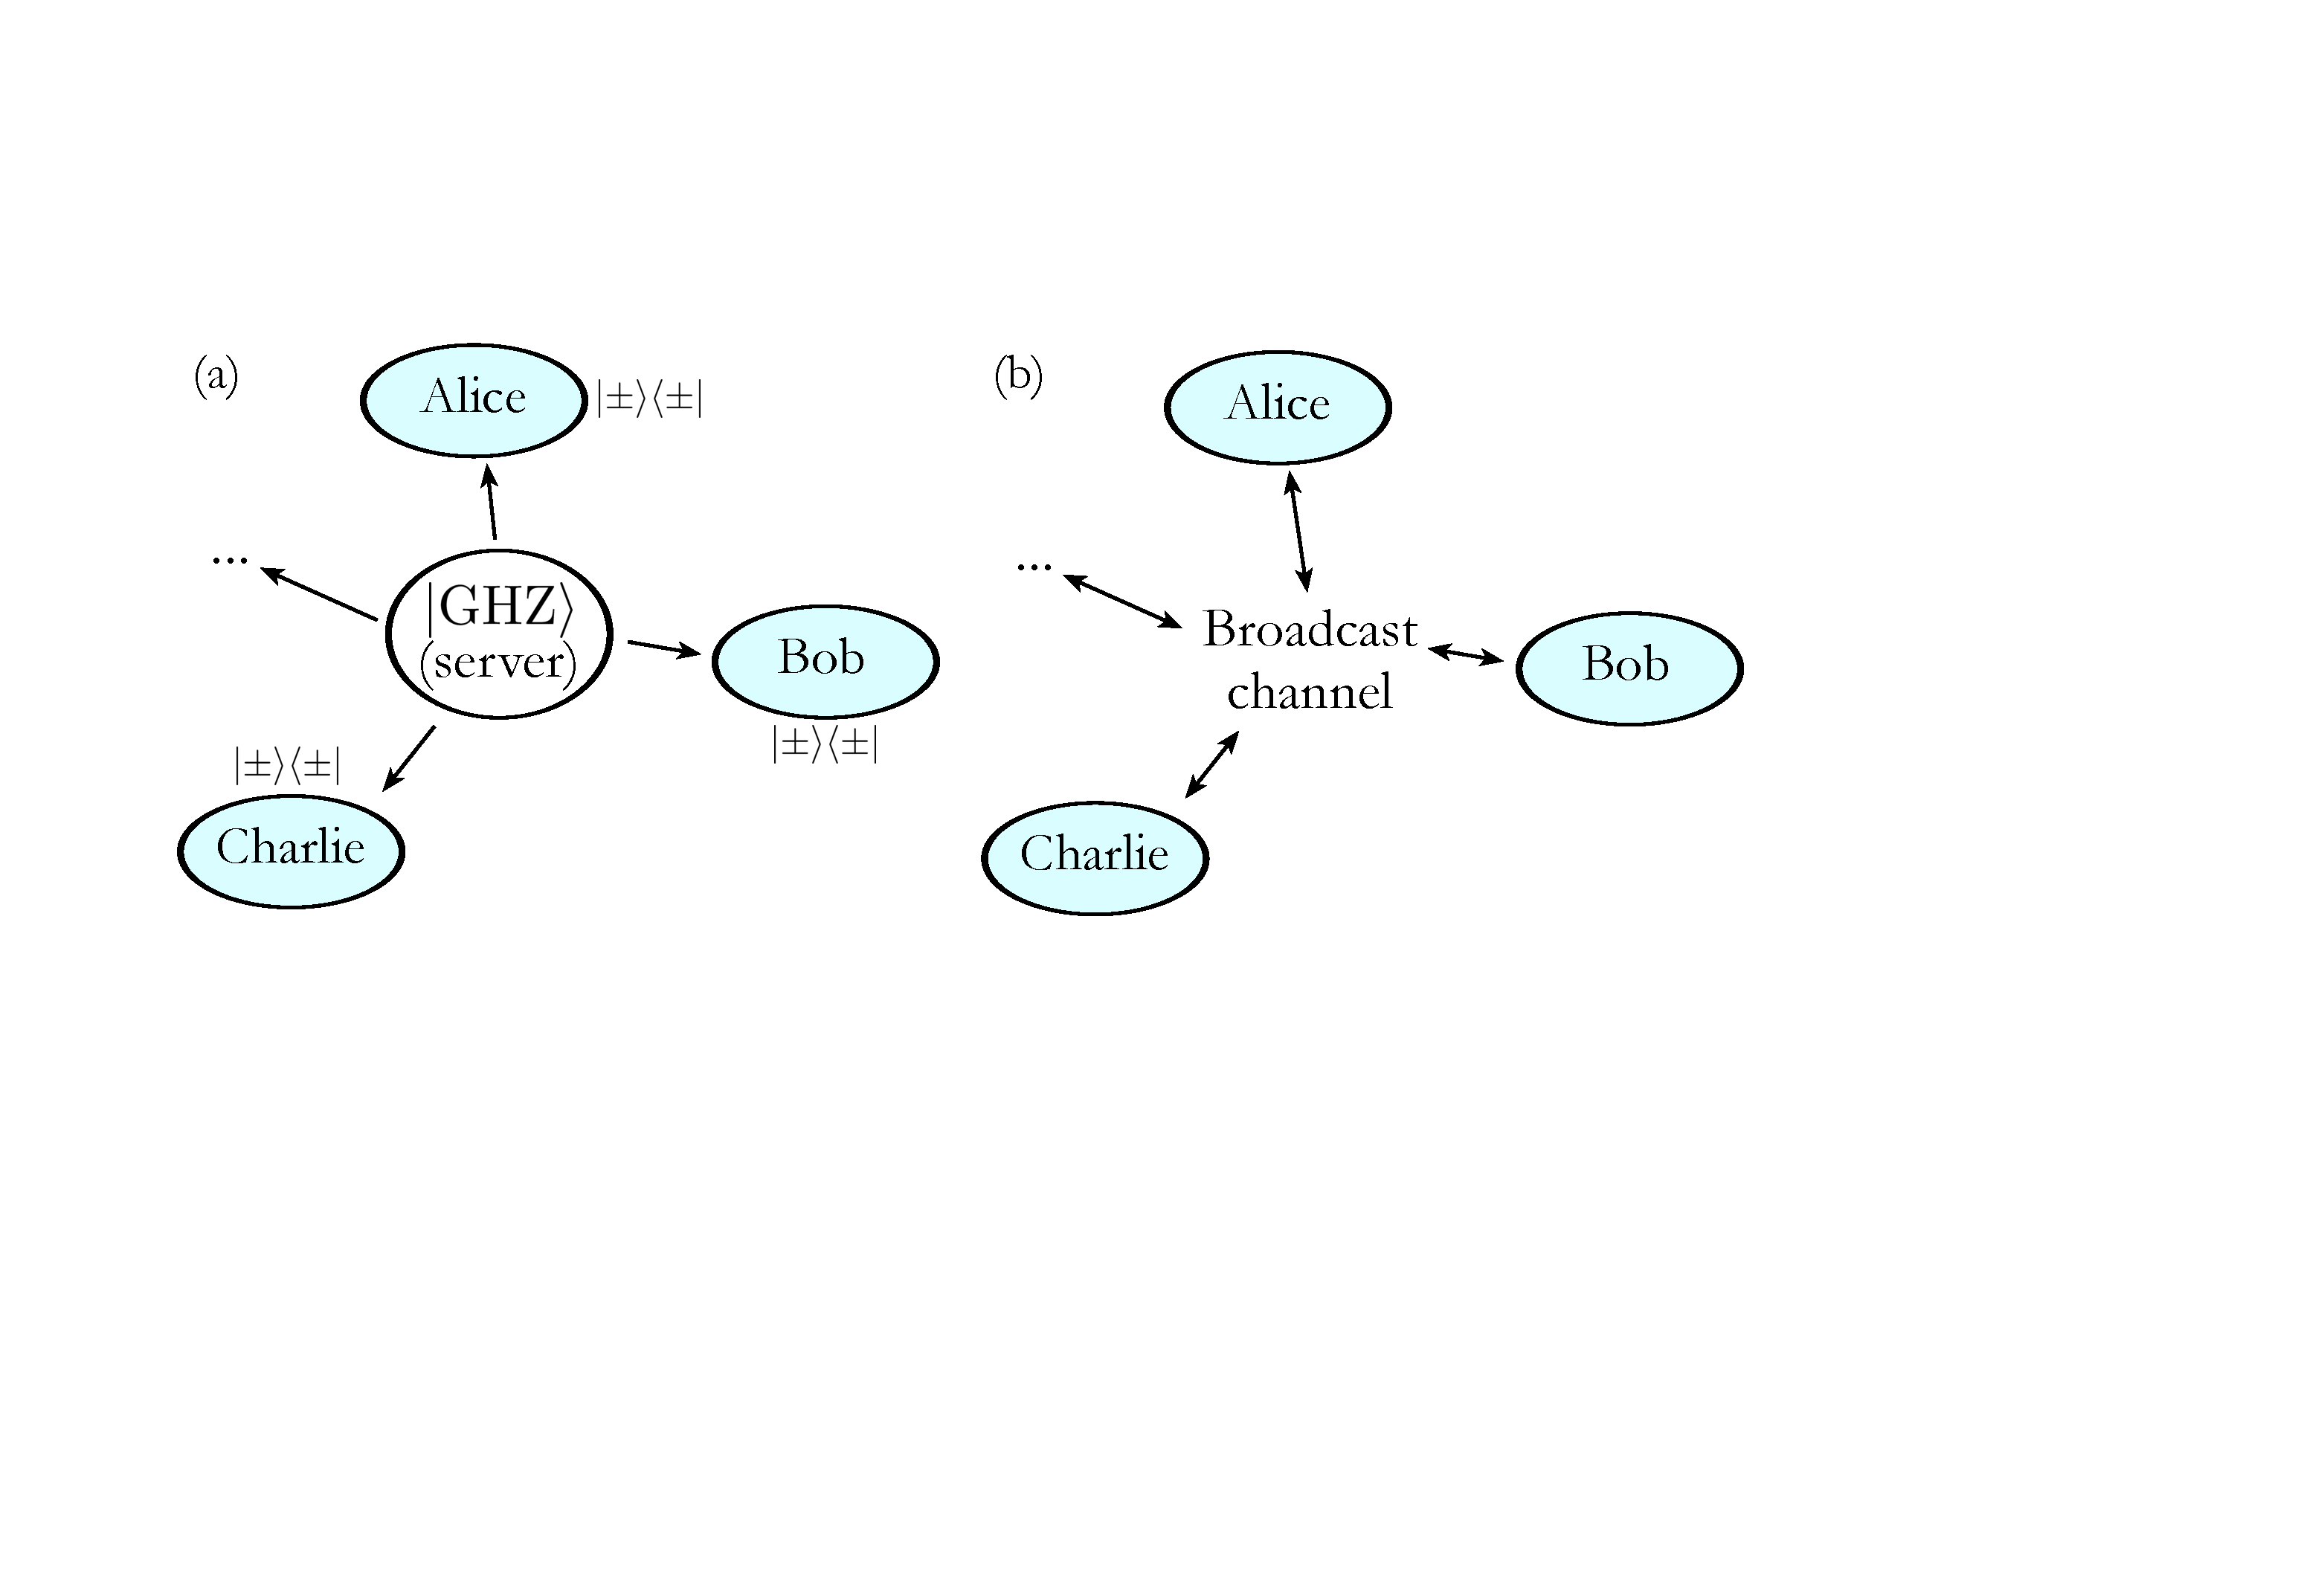
\includegraphics[width=0.47\textwidth]{QAB}
\caption{Protocol for quantum anonymous broadcasting. (a) A central trusted server prepares GHZ states and distributes them amongst a group of users, one qubit per user. All uses measure in the $\pm$-basis. (b) All users classically broadcast their measurement outcomes yielding shared random parity. During broadcast, the broadcaster lies about his measurement outcome to flip the joint parity if he wishes to transmit `1', or tells the truth to transmit `0'. The joint parity encodes the message of the anonymous user, which all listeners are able to recover.} \label{fig:QAB}	
\end{figure}

\begin{table}[!htb]
\fbox{\parbox{0.965\columnwidth}{\texttt{ 
function QuantumAnonymousBroadcasting(message, speaker):
\begin{enumerate}
\item $\ket\psi = \ket{\mathrm{GHZ}}$
\item $\ket\psi \to (\hat{Z}_\mathrm{speaker})^\mathrm{message}\ket\psi$
\item for(i$\in$users) \{
	\setlength{\itemindent}{.2in}
\item outcome$_i$ = measureInXBasis($\ket\psi_\mathrm{i}$)
\setlength{\itemindent}{0in}
\item \}
\item parity = $\sum_i$ outcome$_i$\,(mod\,2)
\item return(parity)
\item $\Box$
\end{enumerate}
}}}
\caption{Protocol for quantum anonymous broadcasting. The GHZ state is distributed in advance, one qubit per user. The measurement outcomes are classically broadcast without encryption. The final parity of the classical measurements reflects the message bit without identifying the speaker.} \label{alg:QAB}
\end{table}

Note that the scheme can be slightly simplified by rather than the speaker applying the $\hat{Z}$ to his qubit, upon announcing his measurement outcome he instead lies about his outcome and flips it. This follows simply because a $\hat{Z}$ gate prior to a $\pm$ measurement bit flips the classical measurement outcome, \mbox{$\hat{Z}\ket\pm=\ket\mp$}.

There are no constraints on time ordering of the measurements, nor, much like BB84, are there any interferometric requirements (not including the GHZ preparation stage), making this protocol very experimentally practical over long distances.

Because of the time invariance in the measurements, distribution and measurement of the GHZ states can be performed well in advance of the actual message broadcast. This allows us to treat `shared parity'\index{Shared parity} as a fundamental resource (Sec.~\ref{sec:ent_ultimate}) for the QAB cryptoprotocol.

Since the parity-sharing can be isolated from the broadcasting stage it is unimportant if the GHZ source is non-deterministic or the channels for distributing it lossy. We can instead simply repeat GHZ distribution over and over at high repetition rate, post-selecting upon measurement outcomes where all users signal that they successfully received and measured their photons.

For these reasons, this scheme lends itself readily to photonic implementation, provided a reliable GHZ preparation circuit. The scheme has since been ported to operate on toric codes\index{Toric code} to facilitate error correction of the distributed GHZ states.

%
% Attacks On Quantum Cryptography
%

\subsection{Attacks on quantum cryptography}

\comment{To do}